\chapter{Hyperledger Fabric}
\section{Introduzione}
Fondata dalla Linux Fondation nel 2015 per anticipare le tecnologie blockchain industriali, Hyperledger Fabric si presenta come standard una singola blockchain, incoraggia un approccio collaborativo per sviluppare tecnologie blockchain attraverso un processo di community, con diritti di proprietà intellettuali che incoraggiano uno sviluppo aperto e dinamico.
Hyperledger Fabric è uno dei progetti open-source basato su blockchain all’interno di Hyperledger. Come altre tecnologie blockchain, ha un ledger, utilizza smart contract, ed è un sistema attraverso il quale i partecipanti gestiscono le proprie transazioni.
Dove Hyperledger Fabric si differenzia da altri sistemi blockchain è che è privato e permissioned. Invece che essere un sistema aperto permissionless che permette a identità sconosciute di partecipare alla rete (richiedendo protocolli quali “proof of work” per convalidare le transazioni e rendere sicura la rete), i membri di Hyperledger Fabric sono iscritti tramite un Membership Service Provider (MSP) di fiducia.
Hyperledger Fabric inoltre offre svariate opzioni innestabili. I dati sono immagazzinati secondo una particolare struttura, i meccanismi di consenso possono essere sostituiti, e sono supportati vari MSP.
Hyperledger Fabric inoltre offre la possibilità di creare canali, permettendo a un gruppo di partecipanti di formare un ledger di transazioni separato. Questa è un’opzione particolarmente importante per le reti in cui alcuni partecipanti potrebbero essere concorrenti e non volere che ogni transazione fatta da loro sia nota a tutti i nodi. Due partecipanti formano un canale, questi due, e nessun altro, possiedono le copie del ledger per quel channel preso da riferimento.
\newpage
\section{Funzionalità di Hyperledger Fabric}
Le funzionalità su cui si basa tale progetto sono quelle legate a blockchain di tipo private e permissioned. Le caratteristiche fondamentali che si affacciano verso questo ambiente sono la modularità, la sicurezza, scalabilità e performance. Le funzionalità principali sono le seguenti:
\subsection{Gestione dell'identità}
La gestione delle funzionalità legate a ogni peer è specificato all'interno di un meccanismo di autenticazione proprio delle blockchain permissioned. Vi è un sistema d'identificazione che riesce ad assegnare a ogni utente connesso alla rete un ID univoco. Tale ID specifica i permessi per accedere a particolari funzionalità del chaincode, alla visibilità su alcune strutture dati e sulla distribuzione di un nuovo chaincode.
\subsection{Privacy e riservatezza}
All'interno della gestione della rete su cui si basa Hyperledger Fabric, vi sono meccanismi di privatizzazioni di alcune transazioni, visibili solamente ai nodi collegati a uno specifico canale privato. L'uso di tali canali stabilisce una privatizzazione delle transazioni che permettono di far sussistere più organizzazioni (aziendali o logiche) su una medesima rete. All'interno delle transazioni noi possiamo gestire la riservatezza sia per i dati e sia per informazioni proprie dei membri o del canale. Questo meccanismo garantisce un principio di riservatezza che in altre blockchain sono inesistenti. Inoltre, riesce a sfruttare la sicurezza degli accessi propria delle blockchain di tipo permissioned e private.
\subsection{Processi efficienti}
Hyperledger Fabric assegna i ruoli di rete a secondo delle tipologie di un nodo. Per fornire concorrenza e parallelismo alla rete, si ha una separazione tra le varie operazioni di gestione delle transazioni tra: esecuzione, applicazione e ordinamento. Eseguire le transazioni prima di ordinarle permette a ogni nodo di processarne più di una simultaneamente. Questa esecuzione concorrente aumenta l’efficienza del processo di ogni peer e accelera la consegna delle transazioni al servizio di ordine che operarà successivamente.
Oltre ad abilitare il processo parallelo, la divisione del lavoro libera i nodi ordinanti dalle richieste di esecuzione delle transazioni e di mantenimento del ledger, mentre i peer sono liberati dal superlavoro di ordine che rappresenta l'operazione di consenso per la validazione delle transazioni. Questa biforcazione di ruoli limita anche il processo richiesto per l’autorizzazione e l’autenticazione; tutti i nodi non devono fidarsi di quelli adibiti al consenso e viceversa. In questo modo i processi su particolari peer possono essere eseguiti indipendentemente dalla verifica degli altri avente come risultato quello di separare i ruoli in maniera modulare.
\subsection{Funzionalità del chaincode}
All'interno di Hyperledger Fabric, i chaincode sono utilizzati per definire una logica di business per tipi di transazione propri per un canale, essi specificano la logica per la gestione della strutturazione dei dati e della loro manipolazione. Poichè le transazioni sono proprie di un canale, tutte quelle di una medesima tipologia seguiranno le regole specificate dallo smart contract proprio della sotto-rete (channel). L'altra forma di chaincode ha come scopo principale quello di definire le regole di validazione delle transazioni. 
\subsection{Modularità di Hyperledger Fabric}
Hyperlegder Fabric implementa un’architettura modulare per fornire una scelta funzionale ai progettisti della rete. Algoritmi specifici per l'identificazione, l'ordinamento (definito anche come meccanismo di consenso) e gestione della crittografia, per esempio, possono essere configurati programmaticamente all'interno di ogni rete basata su Fabric. Il risultato è una architettura blockchain universale che ogni industria o dominio pubblico può adottare e personalizzare.
\newpage
\section{Principi su cui si fonda Hyperledger Fabric}
Hyperledger Fabric ha un modello dinamico, incentrato sulla variabilità nella configurazione di alcuni concetti fondamentali che definiscono i punti cardine su cui si appoggi la struttura. Secondo una visione ad alto livello, essi si possono sintetizzare nei seguenti aspetti:
\begin{enumerate}
    \item Privacy: tramite l'utilizzo di collezioni di dati e canali privati, possiamo definire un meccanismo di riservatezza in cui le informazioni di una transazione sono visibili solamente ai soli nodi collegati a un canale. Con tale meccanismo, Hyperledger Fabric soddisfa le richieste di riservatezze dei dati cosi da poter mantenere su una medesima rete più organizzazioni.
    \item Sicurezza: basandosi su una blockchain di tipo permissioned, i nodi che sono all'interno della rete sono autenticati e registrati dentro il MSP (Membership Service Provider). Inoltre, le transazioni sono rilevabili ai soli nodi autorizzati alla visione e alla validazione del loro contenuto.
    \item Consenso: dando dinamicità e flessibilità di gestione all'interno di un unico meccanismo di approvazione e, andando a definirne le caratteristiche in maniera programmatica, si ha un aumento dell'efficienza del sistema di verifica delle transazioni.
\end{enumerate}
\newpage
\section{Componenti funzionali alla base del modello}
All'interno di tale paragrafo andremo a definire una panoramica approfondita delle componenti che vengono utilizzate per il funzionamento di Hyperledger Fabric andando a descrivere le caratteristiche principali per ciascun elemento. Andremo anche a ridefinire alcuni concetti noti all'interno del contesto delle blockchain cosi da poter sottolineare come le funzionalità di tali elementi si adattino al modello offerto da Hyperledger Fabric.
\subsection{Ledger}
Il ledger è una delle componenti principali che si identificano all'interno 
\newline dell'architettura su cui si fonda Hyperledger Fabric. Per definizione, esso non fa altro che mantenere in maniera immutabile una catena d'informazioni inerenti a tutti i passaggi di stati che si sono avuti all'interno della storia della rete su cui si appoggia. In altri termini, mantiene la storia degli stati precedenti e di quella attuale della blockchain. Una transizione di stato si ha quando si invoca un chaincode susseguita dalla creazione e l'esecuzione di una transazione. Vi è un ledger per ogni canale presente sulla rete. Tale ledger è strutturato come una catena di blocchi in cui ogni blocco ha un numero definito di transazioni formate da record con coppie di chiave-valore, inoltre si mantiene uno stato corrente del database in cui sono memorizzati i dati. Poichè il ledger è proprio di un canale e ognuno di essi ha dei membri rappresentati da alcuni peer della rete, per la natura distribuita su cui si fonda Hyperledger Fabric, si ha una distribuzione di una copia del ledger all'interno di ogni nodo che è membro del canale. A ogni transazione, si avrà una transizione di stato che andrà ad aggiornare ogni copia del ledger. Quando si effettua una transazione, si va a operare solamente sulle informazioni contenute all'interno dell'ultimo blocco aggiunto della catena che rappresenta lo stato globale corrente. Tale stato mantiene tutti in valori dei dati che sono visibili a un canale e, di conseguenza, a ciascuno dei suoi membri. Per manipolare lo stato e i dati correnti annessi, Hyperledger Fabric si appoggia su un database che mantiene tutte le informazioni manipolabili. All'interno di tale database sono presenti solamente i dati dello stato corrente e non quelli della storia passata in modo da garantire l'immutabilità propria della blockchain. Il tipo di un database di stato segue una delle seguenti opzioni di 
\newline
\begin{itemize}
    \item LevelDB: rappresenta il database di stato per default, vi sono tante copie distribuite tra i vari membri del canale. I dati sono mantenuti come una sequenza di coppie chiave-valore.
    \item CouchDB: rappresenta un database di stato alternativo basato su una struttura JSON, tale database riesce ad aumentare l'efficienza tramite l'utilizzo di numerose query sui meta-dati codificati sempre in linguaggio JSON e propri del chaincode di riferimento.
\end{itemize}
La scelta di tale configurazione per la persistenza di uno stato è definita programmaticamente all'interno della configurazione dell'architettura del sistema.
\subsection{Smart Contract e Chaincode}
All'interno di Hyperledger Fabric, i chaincode e i ledger costituiscono il cuore della piattaforma. Il ledger definisce tutta la storia dei stati passati e correnti di un oggetto di business, i chaincode definiscono la business logic eseguibile su di essi per la variazione del loro stato. I chaincode non vengono solamente utilizzati per operazioni di transizione su strutture dati interne al canale in cui si è effettuato il deploy, ma anche per definire caratteristiche a basso livello proprie di Fabric. Prima di definire una transazione, bisogna specificare e caricare uno smart contract in modo da poter precisare dati, concetti e processi. Presi insieme, formano il modello di business su cui si basa la comunicazione tra le parti interessate nel completamento della transazione. Usando una rete blockchain, possiamo definire uno smart contract all'interno di programmi eseguibili in modo da poter operare su degli oggetti di business che verranno utilizzati internamente a una transazione. Hyperledger Fabric utilizza i termini smart contract e chaincode in maniera intercambiabile. In generale, uno smart contract definisce la logica transazionale che controlla il ciclo di vita di un oggetto di business contenuto all'interno dello stato globale della rete. Configurazione:
\newline
\newline
In relazione al ledger, uno smart contract accede a due sue parti: la blockchain, andando a poter visualizzare tutte le transazioni effettuate all'interno della rete e uno stato globale che mantiene una cache con i valori correnti di tutti i dati globali e degli oggetti di business del network. In relazione allo stato globale, uno smart contract può compiere tre operazioni principali:
\begin{enumerate}
    \item GET: Che prende delle informazioni tramite query all'interno del database in cui sono immagazzinati i valori che costituiscono lo stato globale. 
    \item PUT: Che crea un nuovo oggetto di business andandolo a inserire all'interno dello stato globale del ledger.
    \item DELETE: Che cancella un oggetto di business all'interno dello stato globale del ledger ma non nella sua storia, ossia esso non sarà più presente nello stato corrente ma la blockchain traccerà sempre le transazioni passate effettuate su tale entità, andando a mantenere la caratteristica d'immutabilità propria dei suoi blocchi.
\end{enumerate}
Per effettuare tali operazioni di base, Hyperledger Fabric si avvale dell'uso di specifiche API. Inoltre, esse sono di fondamentale importanza se all'interno del modello di business vi sono procedure che interessano la lettura, scrittura o la cancellazione di dati, che essi siano persistenti o di sessione.
Un altro aspetto legato a ogni chaincode sono le regole di approvazione (endorsement). Esse sono molto importanti perchè definiscono quali organizzazioni devono firmate una transazione generata da un determinato smart contract in modo tale da poterla considerare valida. Ogni transazione sottomessa viene aggiunta al ledger distribuito ma solamente quelle valide andranno ad aggiornare lo stato globale.
\begin{figure}[h]
    \centering
    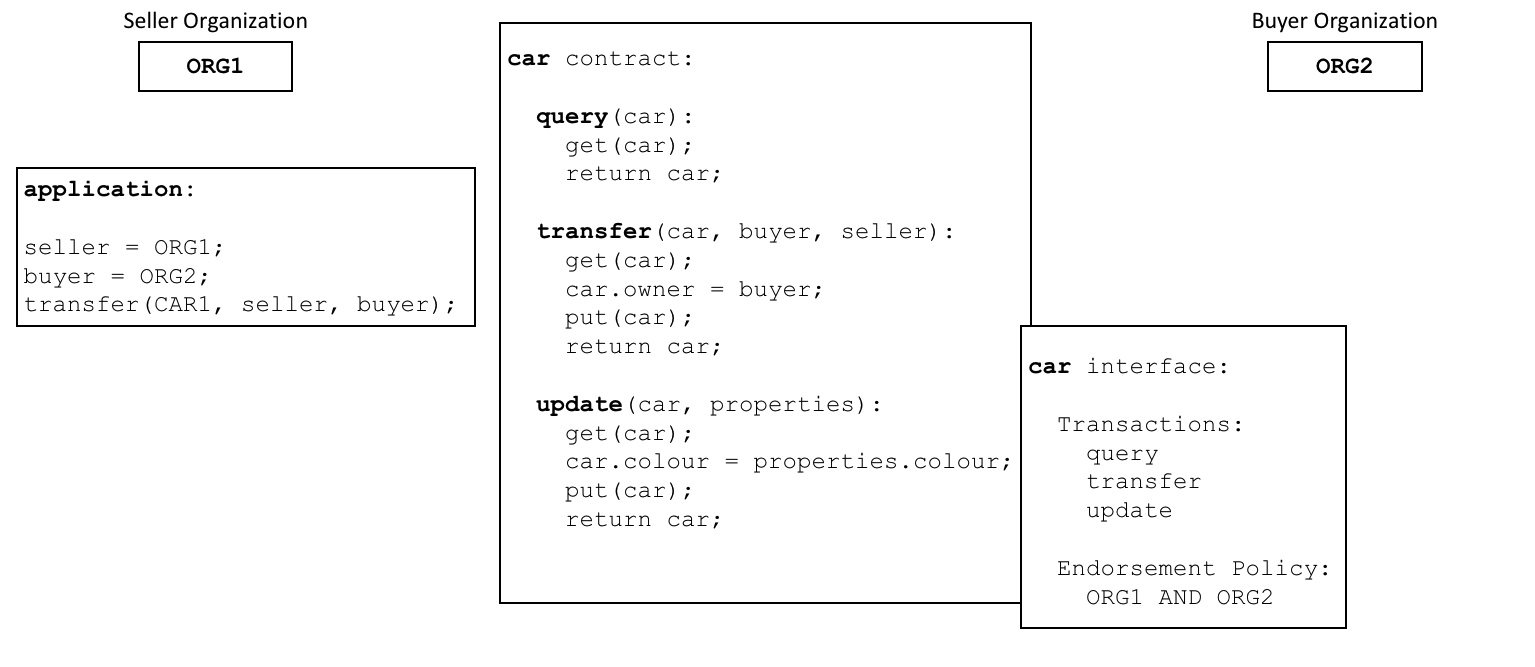
\includegraphics[width=1\textwidth]{img/endorsement.png}
    \caption{Applicazione di un trasferimento di proprietà di un auto}
    \label{fig:endorsement-policy}
\end{figure}
Le regole di endorsement sono una delle caratteristiche che distingue Hyperledger Fabric dalle altre piattaforme legate alle reti di tipo blockchain. Grazie a queste regole, ogni nodo può generare una transazione, ma essa deve essere sempre verificata da specifiche organizzazioni che, rispetto alle classiche blockchain come Bitcoin ed Ethereum, sono definite in un contesto incentrato su una logica che modella più realisticamente il mondo reale. Dato che Hyperledger Fabric si basa su una permissioned blockchain, le regole di approvazione definiscono anche le organizzazioni legate alla validazione delle transazioni, ossia quei nodi che, all'interno della rete, sono considerati affidabili in modo da poter verificare la correttezza delle operazioni eseguite sul network. Le politiche di approvazione sono solamente una delle varie tipologie di regole che si ha all'interno di Fabric, è possibile anche definire dei criteri per la cancellazione e modifiche di dati, oppure per la definizione di quali nodi possono effettuare particolari operazioni di business su specifici oggetti dello stato globale. In tutti i casi, le regole dovrebbero essere concordate all'interno del consorzio delle organizzazioni prima di effettuare una transazione sulla blockchain. In Hyperledger Fabric, ogni tipo di policy può essere programmaticamente modificata rispetto alla forma standard, i meccanismi di aggiornamento delle regole sono anche loro dei criteri di gestione che sono definite all'interno del dominio delle policy della piattaforma. Tramite le politiche di modifica, possiamo anche modificare la logica di endorsement della blockchain su cui si fonda il nostro software. 
Un'altra delle caratteristiche principali sull'utilizzo dei smart contract all'interno del contesto basato su Hyperledger Fabric è il meccanismo di validazione di una transazione mediante l'uso di una proposta transazionale. La procedura di esecuzione di una proposta è eseguita all'interno dell'istanza di un chaincode in un peer dell'organizzazione seguendo le politiche di approvazione proprie del ledger, i valori contenuti all'interno dello stato globale e la logica di business definita nel codice dello smart contract. La risposta alla proposta di transazione è costituita da un set di dati lettura e scrittura, che identificano le informazioni lette dallo stato globale e quelli da scrivere o aggiornare in seguito all'applicazione della transazione. Lo stato globale non viene modificato durante la proposta poiché la transazione deve essere ancora validata. 
\begin{figure}[h]
    \centering
    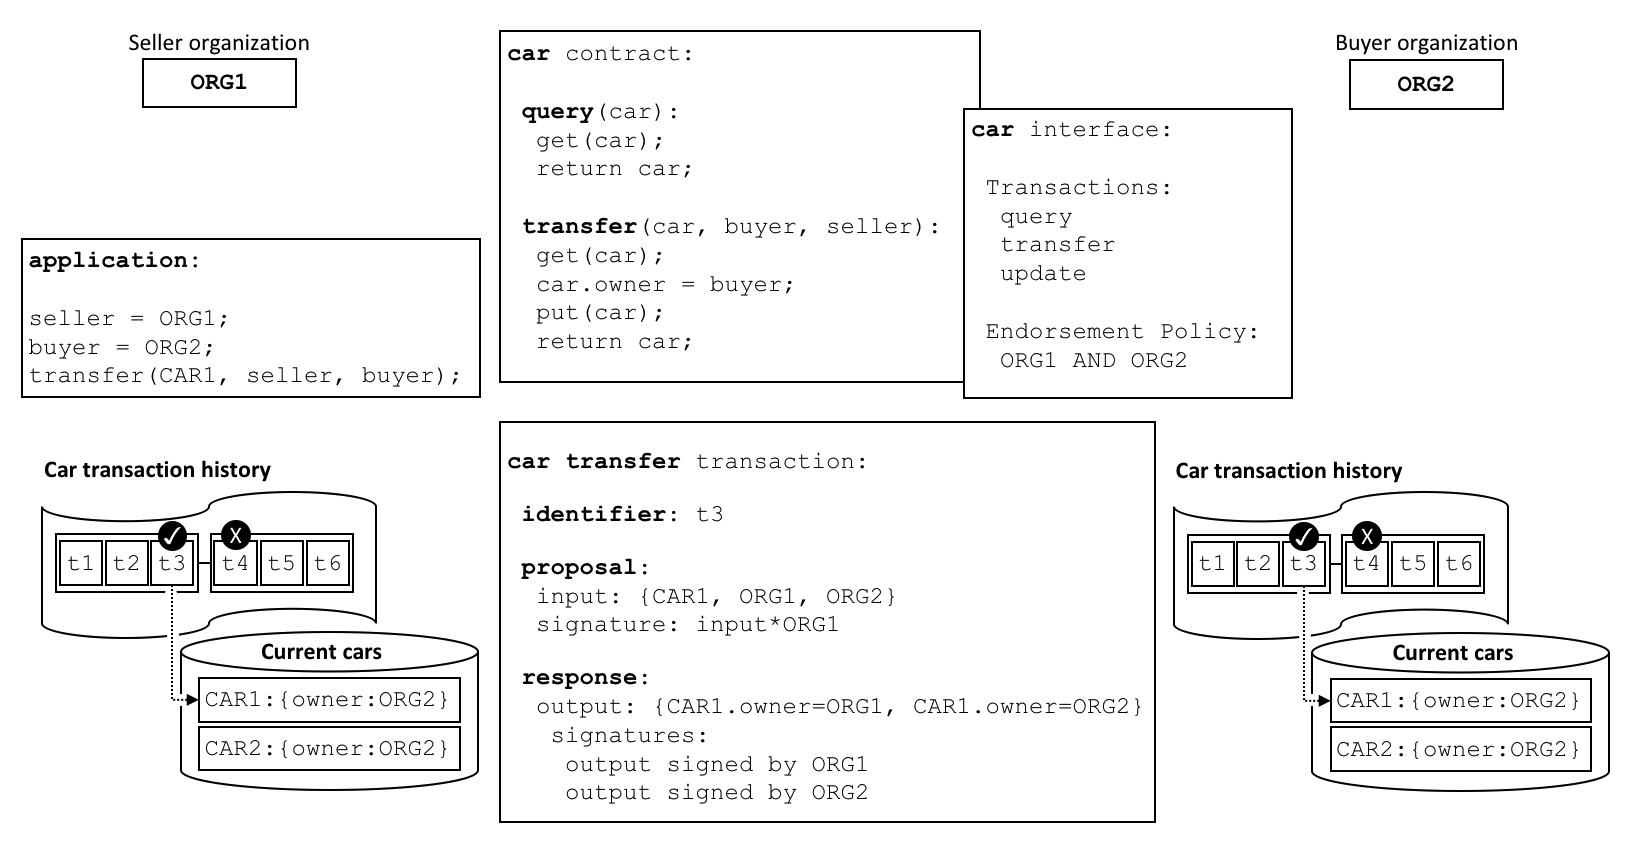
\includegraphics[width=1\textwidth]{img/transaction-proposal.png}
    \caption{Procedimento di una proposta di transazione basata sul caso 3.1}
    \label{fig:transaction-proposal}
\end{figure}
Trovandoci in un ledger distribuito, le transazioni devono essere propagate a tutti i peer di una rete. Prima di ciò, una transazione deve essere sottomessa a due fasi di convalida:
\newpage
\begin{enumerate}
    \item La prima fase si assicura che la transazione è stata verificata con successo dalle organizzazioni specificate all'interno della politica di approvazione legata allo smart contract. 
    \item La seconda fase verifica che lo stato globale corrente sia uguale a quello visualizzato dai peer di convalida nella fase di validazione della transazione, cosi da evitare di modificare i dati nel caso si sono effettuati degli aggiornamenti intermedi.
\end{enumerate}
Se la transazione sotto esame supera queste due fasi di verifica, viene contrassegnata come valida andando a modificare sia lo stato globale e sia la storia della blockchain. In caso non si soddisfi una delle due fasi, la transazione non andrà a modificare i valori dello stato globale ma verrà comunque annessa alla storia della blockchain.
\begin{figure}[h]
    \centering
    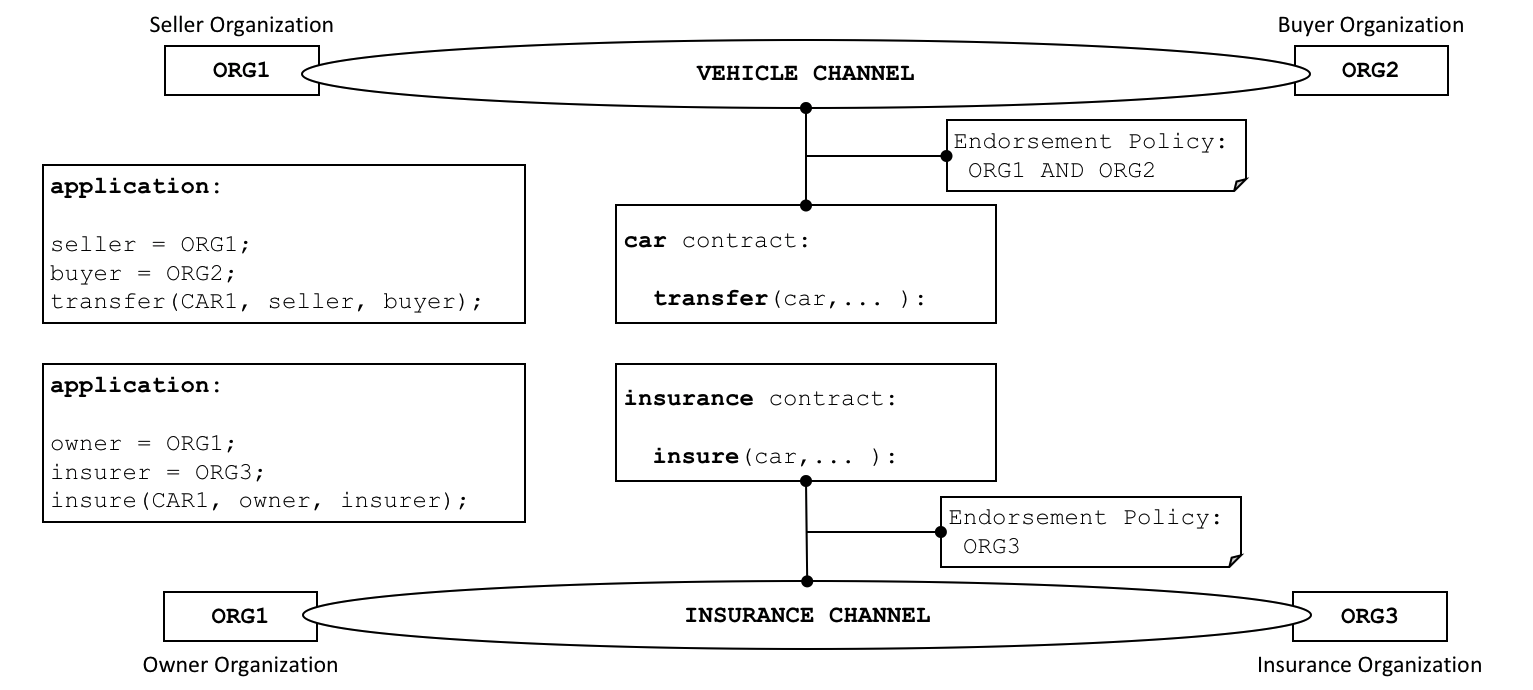
\includegraphics[width=1\textwidth]{img/channel-transaction.png}
    \caption{Architettura di esempio con canali annessi}
    \label{fig:channel-transaction}
\end{figure}
Hyperledger Fabric ha la capacità di poter stabilire più canali indipendenti cosi da riuscire a dividere collezioni e processi di una medesima organizzazione in relazione a controparti differenti e, allo stesso tempo, poter coordinarne le attività dipendenti. Ogni canale dispone di un proprio smart contract che ne definisce la struttura delle transazioni andando a definirne dati, operazioni logiche e parti interessate. A ogni smart contract si ha una politica di approvazione differente e dipendente unicamente dal canale e dai suoi partecipanti. Strutturati in questo modo, i canali rappresentano una propria blockchain. Una medesima organizzazione può essere partecipe in più blockchain senza nessuna restrizione. 
Gli smart contract vengono utilizzati in Fabric anche per la gestione di funzionalità a basso livello indipendenti dai processi aziendali delle organizzazioni presenti sulla rete.
Questi smart contract vengono definiti come chaincode di sistema, e possono essere di uno dei seguenti tipi:
\begin{enumerate}
    \item Lifecyrcle  System Chaincode (LSSC): definisce uno smart contract che gestisce la firma del pacchetto, l'installazione, la creazione di istanze e l'aggiornarnamento delle richieste di un chaincode. 
    \item Configuration System Chaincode (CSCC): istanziato su ogni peer, definisce i meccanismi di gestione e di aggiornamento dei criteri propri di un canale. 
    \item Query System Chaincode (QSCC): Definisce delle query che andranno a comporre le API del ledger per definire delle operazioni su singole transazioni o su interi blocchi della blockchain.
    \item Validation System Chaincode (VSCC): definisce la politica di approvazione, i criteri di strutturazione del set di lettura e scrittura per la verifica dello stato in fase di convalida e le organizzazioni interessate alla validazione di una transazione. 
    \item Endorsement System Chaincode (ESCC): fornisce un supporto ai peer per le firme crittografiche su una transazione.  
\end{enumerate}
Le modifiche ai chaincode di sistema è un processo molto delicato e vulnerabile ai cambiamenti. Essendo una attività molto specifica, un'implementazione scorretta può portare a delle malfunzionalità di alcuni peer come, ad esempio, il voler aggiornare un Validation System Chaincode in maniera differente in più peer di una medesima organizzazione andandone ad alterare il meccanismo del consenso della blockchain sottostante creando eventi come il forking.
\subsection{Peer}
I peer sono le fondamenta di una rete di tipo blockchain. Rappresentano l'unità computazionale capace di poter eseguire processi in maniera distribuita all'interno di una rete. Ogni peer ha una propria copia del ledger e una medesima istanza di un chaincode. Hanno un ciclo di vita indipendente da quello della rete. Possono essere facilmente creati, eseguiti, messi in pausa, riconfigurati oppure cancellati tramite apposite APIs proprie degli amministratori del sistema.
\begin{figure}[h]
    \centering
    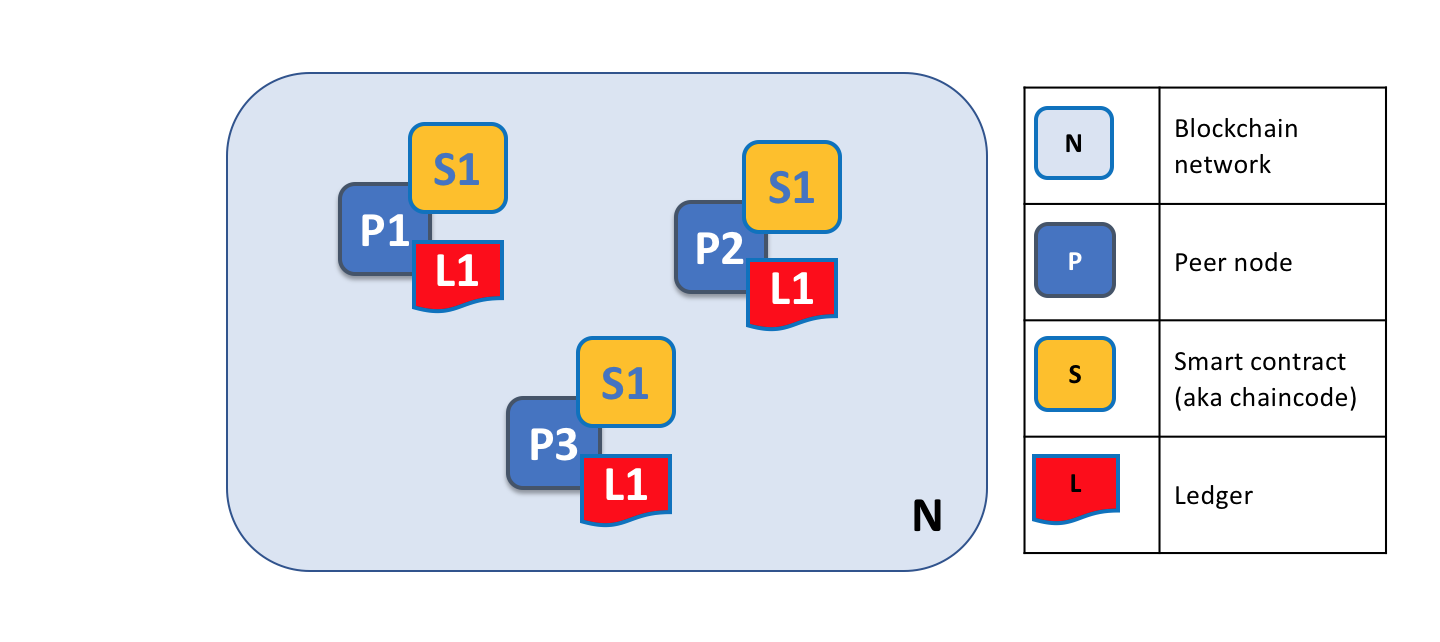
\includegraphics[width=1\textwidth]{img/peer-diagram.png}
    \caption{Visione logica dei peer}
    \label{fig:peer-diagram}
\end{figure}
Notiamo che all'interno di un peer non vi sono chaincode e ledger ma istanze di quest'ultime. Tale caratteristica può prevedere, quindi, che all'interno di un singolo peer vi siano più istanze di chaincode e di ledger. Questo meccanismo offre la possibilità di avere ridondanza che è uno dei principi su cui si fondano i sistemi distribuiti andando ad aumentare anche l'affidabilità delle funzionalità legate a tali elementi. Poichè i peer sono degli host in cui sono localizzate ed eseguite componenti come ledger e chaincode, per poter accedere a questi elementi, bisogna entrare prima al peer che ospita tali istanze. In genere è possibile avere anche istanze differenti di ledger su un medesimo peer, questo garantisce l'interoperabilità tra più ledger distribuiti. Per poter interagire con le istanze dei ledger di un peer, su di esso vanno installati anche i chaincode di riferimento. Tali istanze possono essere assenti anche se configurazioni di questo tipo non sono presenti nei sistemi moderni; questo perchè senza un chaincode di riferimento, il peer non può interagire con il ledger.Notiamo che anche se non vi sono istanze di chaincode per determinare il modello di business su un particolare ledger, all'interno di un peer, per default, vengono sempre installati dei chaincode di sistema per la gestione a basso livello delle funzionalità principali note per la blockchain.
I peer sono dei componenti propri della rete blockchain su cui si fonda Hyperledger Fabric. Tali elementi possono interagire con applicazioni esterne in modo da poter funzionare da mezzo per la gestione delle transazioni sulla blockchain sottostante. La gestione dei peer in relazione alle applicazioni esterne è configurabile programmaticamente tramite l'utilizzo di un SDK dedicato per Hyperledger Fabric. Tramite tale SDK, è possibile gestire i peer e gli altri delle componenti della blockchain tramite l'utilizzo d'interfacce funzionali dedicate. L'interazione tra i peer e le applicazioni esterne non è molto complessa. Il meccanismo di comunicazione può essere riassunto nei seguenti punti:
\begin{enumerate}
    \item L'applicazione si connette al peer all'interno della blockchain
    \item Si invoca una proposta di transazione sull'istanza del chaincode localizzata sul peer che richiama l'istanza del chaincode che esegue l'invocazione richiesta dall'applicazione sui dati dello stato globale del ledger e ritorna una risposta alla query sottomessa. 
    \item L'applicazione riceve la risposta della proposta di transazione, se ha esito negativo termina con uno status di errore interno.
    \item L'applicazione sottomette la transazione all'orderer del canale interessato alla transazione.
    \item L'orderer invia la transazione ai peer in blocco. 
    \item Ogni peer che riceve la transazione aggiorna la propria istanza del ledger andando ad inserire il blocco inerente alla transazione che si è stata effettuata cosi da aggiornare anche la blockchain e lo stato globale. 
\end{enumerate}
\begin{figure}[h]
    \centering
    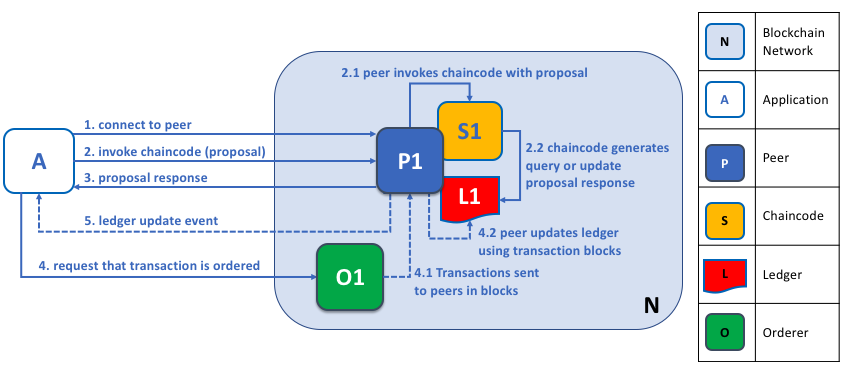
\includegraphics[width=1\textwidth]{img/peer-transaction.png}
    \caption{Transazione sul ledger}
    \label{fig:peer-transaction-process}
\end{figure}
Tutto il procedimento d'invocazione e gestione di una transazione in relazione con un peer, è vista graficamente all'interno della figura 3.5.
Notiamo che una transazione come quella di appena descritta, è propria di tutte quelle operazioni che riguardano l'invocazione di una query all'interno dei dati dello stato globale dell'istanza di un ledger distribuito dentro un peer. La gestione dell'aggiornamento e della manipolazione dei dati distribuiti è data dall'orderer che, come vedremo dopo, è una delle componenti principali per la sottomissione e la manipolazione dei blocchi della catena affiliata a un ledger. Un procedimento simile e più complesso lo si vede, invece, quando al posto di effettuare una query, l'applicazione esterna effettua un aggiornamento dei dati. Questo aggiornamento ha come obiettivo finale quello di andare a effettuare una transizione di stato per qualche oggetto di business del ledger. Tale meccanismo prevede che all'interno dell'aggiornamento del ledger alla fine della sottomissione della transazione, bisogna attendere che tutti i peer di approvazione verifichino la validità della transazione prima di aggiornare effettivamente il ledger, tale politica di acconsenso è verificata con l'uso di ulteriori transazioni che propagano una serie di proposte di aggiornamento a tutti i peer del network. Questa funzionalità è garantita grazie all'impacchettamento delle proposte di aggiornamento in un blocco che viene distribuito a tutti i peer della rete. Se le transazioni di tale blocco vengono verificate dai nodi di approvazione, si passa alla modifica effettiva delle singole copie del ledger all'interno di ciascun peer della rete.
La comunicazione tra i peer avviene per mezzo di un canale. Un canale riesce a mantenere una medesima visione del ledger per un nodo orderer, dei nodi peer e possono interagire anche con applicazioni esterne alla blockchain. La peculiarità principale nell'utilizzo di un canale è data dalla gestione di un medesimo ledger distribuito e per la restrizione della condivisione di dati ai soli peer che sono collegati a tale canale.


\begin{figure}[h]
    \centering
    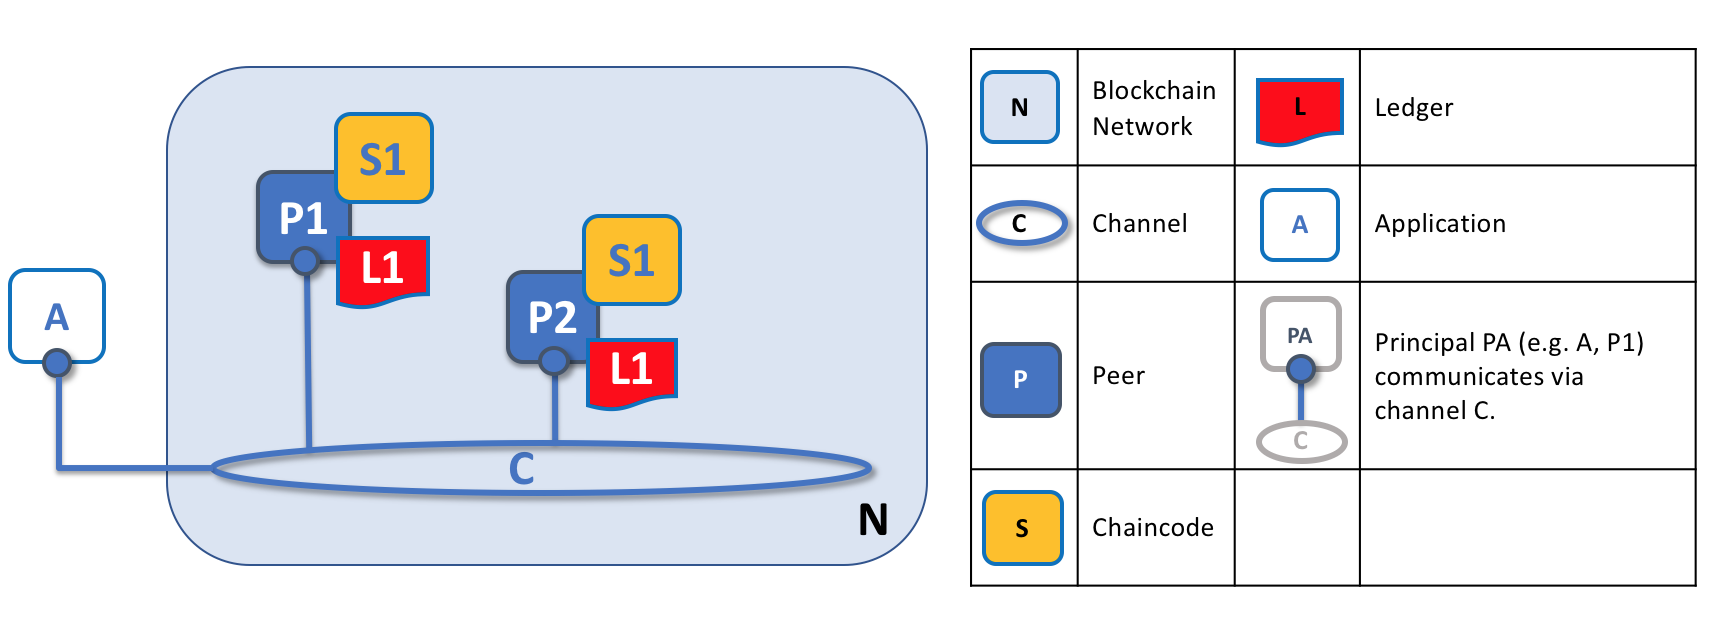
\includegraphics[width=1\textwidth]{img/channel-peer-com.png}
    \caption{Utilizzo di un canale}
    \label{fig:channel-peer-diagram}
\end{figure}
Un altro importante aspetto che riguarda i peer è la loro composizione in gruppi logici chiamati organizzazioni. Le organizzazioni sono un insieme di peer che elaborano delle richieste provenienti, in genere, da una medesima applicazione esterna. I peer che sono propri di un'organizzazione possono anche essere annessi a canali differenti, questo significa che un'organizzazione può collegarsi a più canali e avere visione e gestione di altre transazioni secondo un modello basato sulla privatizzazione delle interazioni e dei dati. Oltre al servizio di ordinamento proprio di un canale, tale struttura non prevede un controllo centralizzato. Anche se tipicamente le applicazioni sono uniche per organizzazione, è possibile avere un'organizzazione che comunichi con più applicazioni che comunicano con molteplici organizzazioni. Questa struttura dinamica è garantita dalla caratteristica della procedura da eseguire: se essa riguarda una query, allora l'applicazione in genere si connette solamente ai peer di una singola organizzazione, se essa, però, aggiorna dei dati, per mantenere il consenso, l'applicazione deve dover comunicare la trasmissione della transazione ai vari peer che hanno il ruolo di validatori secondo le politiche di approvazione del ledger distribuito.
\begin{figure}[h]
    \centering
    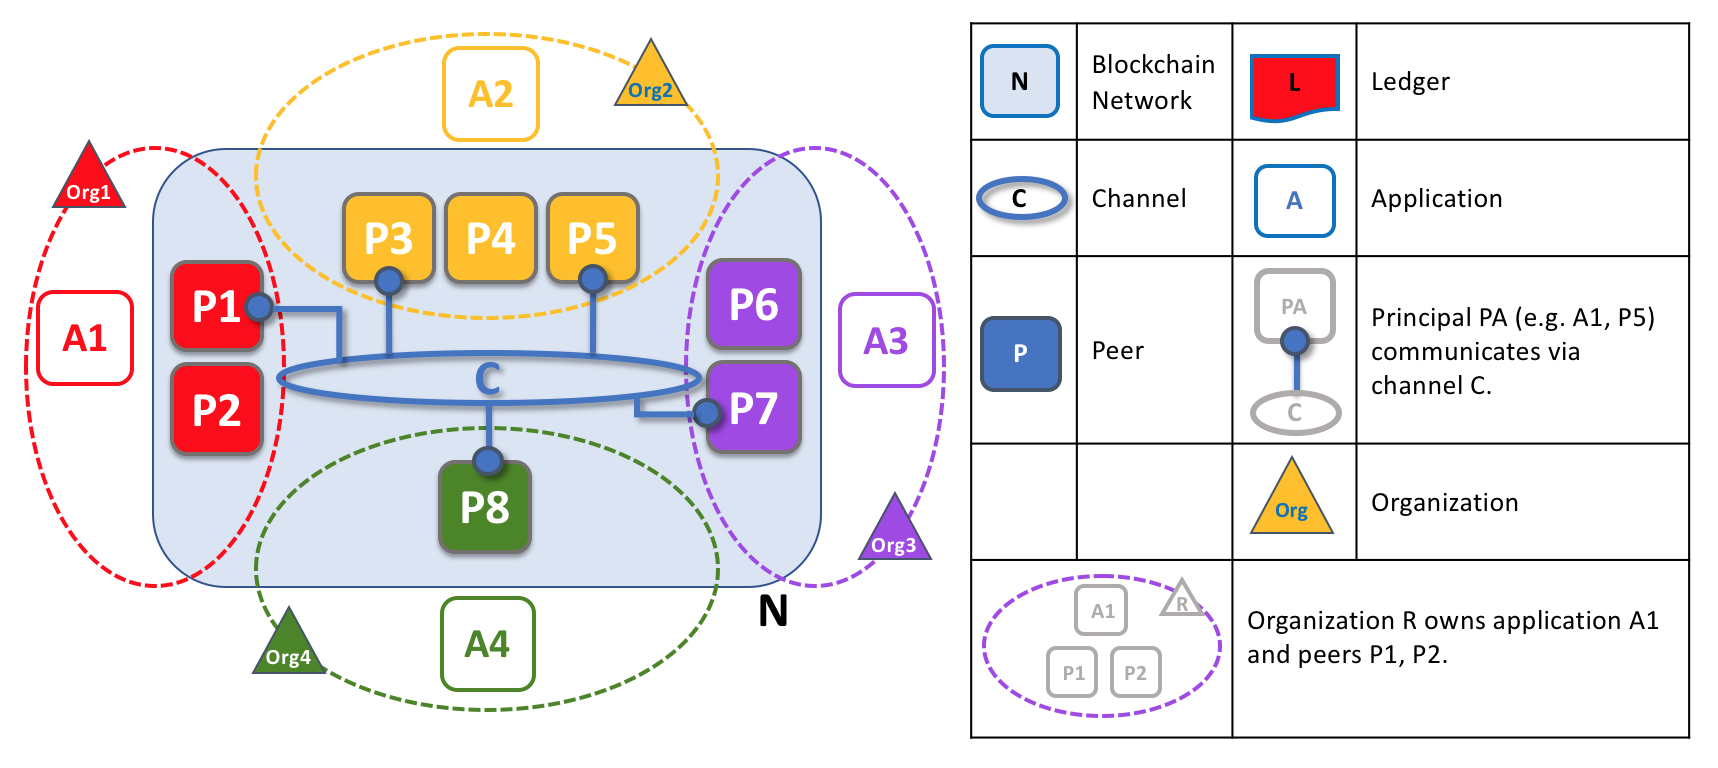
\includegraphics[width=1\textwidth]{img/organization.png}
    \caption{Struttura di una blockchain basata su 4 organizzazioni}
    \label{fig:org-diagram}
\end{figure}
\subsection{Orderer}
Abbiamo visto come i peer possano instanziare ledger e smart contract in modo da poter garantire una interazione con applicazioni esterne mediante lo sviluppo e la gestione di transazioni che vanno a modificare lo stato corrente globale dei dati mantenuti sulla blockchain. Per far si che tutti i peer abbiano la stessa visione dei dati, eseguano le transazioni nello stesso ordine e mantengano uno stato coerente nelle informazioni contenute nella propria istanza del ledger, si ci avvale dell'utilizzo di nodi speciali che vengono definiti come orderer.
Alla base del suo utilizzo vi sono tutte quelle transazioni che vanno ad aggiornare dati del ledger distribuito. Questo perchè se si richiede solamente la lettura dei dati, l'applicazione può co8bmunicare semplicemente con uno dei peer della rete senza dover interpellare altre componenti della blockchain. Invece, quando si tratta di un aggiornamento, si attiva il meccanismo del consenso in cui tutti i peer devono approvare la modifica effettuata e aggiornare i propri ledger. Il procedimento di aggiornamento è molto più lento della procedura che riguarda una semplice query, tale latenza è provocata dalla propagazione della transazione a tutti i peer interessati all'interno della transazione.
Quando si parla di aggiornare un dato all'interno del database di stato del ledger, tutti i peer interessati all'interno della transazione eseguono una procedura di 3 fasi:
\newpage
\begin{enumerate}
    \item Fase di proposta di aggiornamento: un sottoinsieme di peer interessati all'interno della approvazione della transazione, propone una propria versione dell'aggiornamento senza modificare lo stato del proprio ledger.
    \item Fase di impacchettamento: tutte le proposte di aggiornamento vengono impacchettate all'interno di transazioni e inserite all'interno di un blocco. 
    \item Fase di distribuzione e convalida: all'interno di questa fase, l'orderer ha il compito di distribuire a tutti i peer il blocco di transazioni relative all'aggiornamento. Ogni peer andrà a validare le transazioni di tale blocco e, se approvato, verrà aggiornato il ledger distribuito secondo le modifiche delle transazioni proposte. 
\end{enumerate}
Tale procedimento a 3 fasi per l'aggiornamento viene eseguito su blockchain di tipo permissioned. Per altri tipi come Bitcoin ed Ethereum che basano il loro meccanismo di consenso degli aggiornamenti sul Proof of Work, si ha una procedura basata sull'applicazione di un algoritmo di approvazione tipo probabilistico computazionale che, però, sono ancora vulnerabili alla creazione di ledger divergenti tramite forking della blockchain in cui all'interno del proprio ledger vengono accettate le transazioni in ordine differente. In Hyperledger Fabric, invece, tramite l'orderer possiamo ordinare le transazioni e distribuirle per il consenso ai soli peer autorizzati per poi aggiornare tutti i ledger interessati all'interno della blockchain. Tramite l'orderer, l'ordine delle transazioni da accettare è lo stesso e inglobato all'interno di un blocco distribuito cosi da poter eseguire parallelamente l'approvazione su medesime transazioni da parte di più nodi andando ad aumentare l'efficienza e la scalabilità del meccanismo del consenso della blockchain su cui si fonda Fabric. Oltre a organizzare le varie transazioni per la fase di convalida delle transazioni, l'orderer si occupa anche di mantenere traccia di tutte le organizzazioni che hanno i permessi di creazione di un canale. Tali organizzazione formano il consorzio della rete. L'elenco è conservato in un canale di sistema di ordinazione modificabile solamente dall'amministratore dell'orderer. Gli orderer hanno anche il ruolo di amministratori delle operazioni di base che possono compiere i peer delle organizzazioni collegate a un canale andandone a configurare i permessi di accesso, lettura e scrittura ai valori degli oggetti dello stato globale del ledger distribuito. Tali permessi vengono gestiti in fase di convalida di una transazione di aggiornamento proposta da un peer: l'orderer verifica che l'aggiornamento soddisfi i permessi concessi dal peer che ha richiesto la transazione; se approvata, la transazione viene propagata dall'orderer agli altri peer del canale per poi verificare se la transazione soddisfi effettivamente anche le politiche di gestione del canale.
\subsection{Membership Service Provider}
Essendo Fabric una rete blockchain di tipo permissioned, bisogna specificare un meccanismo d'identificazione in modo tale che i peer vengano resi noti in maniera univoca a tutte le altre componenti della rete. Tale meccanismo si raggiunge tramite una procedura basata sull'utilizzo e la distribuzione di chiavi pubbliche all'interno di una blockchain fondata su un meccanismo di fiducia. Le autorità d'identificazione rilasciano in fase di registrazione di un nodo una chiave pubblica, visibile a tutti i peers, e una chiave privata, mantenuta e visibile solamente dal peer proprietario. Poichè la chiave privata non è visibile agli altri peer, si utilizza il Membership Service Provider (MSP) per verificare l'identità di un qualsiasi peer della blockchain. Un esempio della gestione dell'identificazione mediante l'utilizzo del MSP lo si ha nella validazione della firma digitale di una transazione. Quando un peer effettua una transazione, questa viene firmata dal suo creatore mediante la chiave privata, per verificare la validità di tale transazione, ossia che la firma digitale sia effettivamente quella del peer creatore, all'interno del Membership Service Provider viene mantenuto un elenco di tutte le chiavi pubbliche dei peer identificati all'interno della rete.  Notiamo che l'approvazione della transazione ha un alto grado di affidabilità dato che la corrispondenza tra una chiave pubblica e la sua controparte privata è univoca. Il compito di un MSP non si limita a definire solamente l'identità di un peer, ma anche i permessi che ha su un canale a cui è associato definendo cosi anche un ruolo logico rispetto alle operazioni autorizzate che può effettuare. Tale meccanismo è alla base della gestione logica dei dati di Fabric, poiché tramite un MSP è possibile definire i ruoli per singoli peer, organizzazioni o canali. Un MSP definisce i criteri per poter partecipare a una rete autorizzata; essi si concentrano sul soddisfacimento di tali condizioni per i membri della rete:
\newpage
\begin{itemize}
    \item Ottenere una identità da un CA riconosciuto da una rete, ossia acquisire una chiave pubblica e una chiave privata
    \item Far parte ed essere riconosciuto da una organizzazione della blockchain
    \item Aggiungere un MSP al consorzio o al canale
    \item Fare in modo che il MSP sia incluso all'interno delle policy del sistema
\end{itemize}
Sotto un punto di vista implementativo e meno concettuale, un MSP non fornisce nulla, è rappresentato da un insieme di cartelle e file che fanno parte della configurazione strutturale e logica della rete andando a definire le organizzazioni sia internamente (definendo gli amministratori dell'organizzazione) e sia esternamente (definendo meccanismi di validazione delle transazioni andando a rendere partecipi anche peer di altre organizzazioni). Mentre i Certification Authorities sono delle entità che generano delle identità, i MSP sono delle componenti responsabili della loro gestione andando a mantenere la lista delle chiavi pubbliche collegate a ogni ID e utilizzarle per le validazioni di tutte le transazioni aventi come firma quella del peer con l'ID pari a quello preso sotto analisi. All'interno di un MSP si mantiene anche la lista di tutte le Certification Authorities valide in modo da definire un dominio di fiducia di tutte quelle componenti che possono generare delle identità verificate per i membri della rete. Notiamo che un membro della rete non ha solamente un ID univoco che lo contraddistingue, ma anche un ruolo. Tale valore è mantenuto all'interno di un MSP della rete che ha come scopo quello di definire un dominio di operazioni consentite per una particolare entità della rete riuscendo a manipolarle (aggiungere o rimuovere particolari autorizzazioni per uno specifico membro o di una intera categoria).

\subsubsection{Categorie di MSP}
All'interno di una rete blockchain si distinguono due forme di MSP: locali e di canale. In entrambi i casi si hanno le medesime funzionalità, ossia entrambi i tipi di MSP forniscono delle configurazioni di ruoli per ogni identità contenuta al loro interno. La differenza sostanziale che si ha tra le due categorie è l'ambito di applicazioni dei ruoli che definiscono: 

\begin{itemize}
    \item Gli MSP locali vengono definiti localmente all'interno di ogni nodo (peer o orderer) e per i client. Essi definiscono i ruoli in relazione all'ambito applicativo della singola componente (un esempio è quello di definire gli amministratori per un peer oppure chi può operare sul nodo). Gli MSP locali propri dei client, invece, definiscono l'autenticazione per le transazioni sul canale in cui sono membri oppure impostano un ruolo all'interno del sistema come amministratore di una organizzazione. Uno degli obblighi legati a Fabric è quello di dover definire per ogni nodo della rete un MSP locale che definisce chi amministra tale nodo, quale sia la configurazione interna e quali altri componenti hanno diritti di partecipazione sotto quel livello. Altra caratteristica da dover gestire all'interno di un Membership Service Provider all'interno dello scope locale è l'appartenenza a una specifica organizzazione da parte dei nodi aventi come ruolo quello di peer. Cosi facendo, tramite un MSP locale si definiscono amministratori e peer di una organizzazione. Come i peer, anche i nodi con il ruolo di orderer hanno un MSP locale che definisce l'appartenenza a una organizzazione e il dominio di nodi di cui si fida.
    \item Gli MSP globali definiscono i ruoli all'interno dell'ambiente del canale definendone amministratori e partecipanti. Nello specifico definiscono i membri che contribuiscono alla creazione o alla validazione di una transazione propria del canale. Tali MSP definscono le relazioni che vi sono tra le identità e i ruoli dei membri del canale in relazione all'applicazione delle politiche che vi sono su di esso. All'interno di tale MSP vi è la lista degli MSP delle organizzazioni che interagiscono con il canale preso sotto analisi. Ogni organizzazione che interagisce con un canale deve avere un MSP di canale associato, quindi si ha una relazione uno-a-uno tra le organizzazioni che interagiscono con un canale e gli MSP dedicati. Questo perché all'interno di tali MSP si ha la configurazione di come l'organizzazione interagisce con il canale, come viene amministrate, come e quali membri dell'organizzazione partecipano all'interno delle transazioni create internamente al canale. Altro ruolo che si definisce all'interno della configurazione di un MSP di canale è quella della gestione del servizio di ordinamento poiché è possibile avere più orderer che fanno parte di organizzazioni differenti. Tali orderers devono essere configurati per stabilirne una relazione in grado di specificare i meccanismi di consenso e di fiducia per la gestione delle validazioni sul canale. Infine, la memorizzazione di un MSP con scope di canale viene mantenuto, come quello locale, in maniera sincronizzata su più istanze distribuite tra i vari file system dei nodi che interagiscono all'interno del canale.
\end{itemize}
\begin{figure}[h]
    \centering
    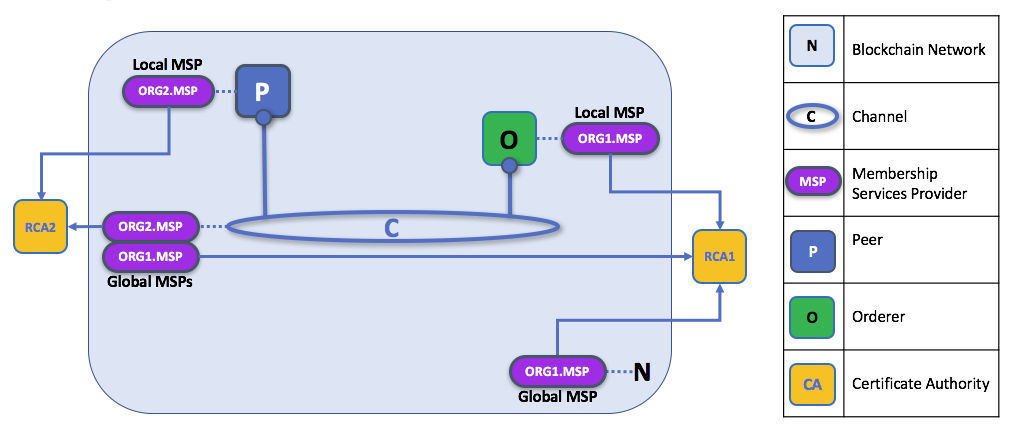
\includegraphics[width=1\textwidth]{img/MSP.png}
    \caption{Architettura di esempio con MSP locali e globali e CA per due organizzazioni}
    \label{fig:msp}
\end{figure}
\newpage
\section{Policy}
Una policy è definita come un insieme di regole che specificano l'infrastruttura per la gestione di un dominio di operazioni eseguite da una particolare o da un gruppo di entità del sistema. In altri termini, definiscono le modalità di accesso, i diritti e come si relazionano delle componenti dell'architettura. Nel caso specifico, le policy su Hyperledger Fabric stabiliscono i criteri di accettazione o di rifiuto di una modifica apportata alla rete, a un canale o a un chaincode. Le policy vengono definite inizialmente dai membri del consorzio, ossia quelle entità in grado di definire la struttura delle componenti di rete (come la creazione di canali). Tale politiche possono essere anche modificate successivamente adottando un approccio evolutivo e dinamico proprio di Hyperledger Fabric.
Le policy è un'altra caratteristica che distingue Fabric da altri tipi di blockchain come Bitcoin ed Ethereum in cui le transazioni possono essere generate e validate da qualsiasi nodo secondo dei criteri fissi con la possibilità di essere modificati solamente in fase d'implementazione andando a modificarne il codice. Hyperledger Fabric, invece, si basa su una blockchain permissioned in cui le policy definiscono la gestione delle transazioni di rete sia in fase compilativa che in quella esecutiva, quali organizzazioni possono accedere e modificare la rete Fabric andandone a specificare anche i metodi applicati, quali organizzazioni possono accedere ad una specifica risorsa come un chaincode di sistema o utente, quali organizzazioni sono interessate per la convalida di una modifica a un canale, di uno smart contract o di una risorsa e i meccanismi di gestione delle firme digitali per la verificabilità di una transazione.
\newpage
\subsection{Tipi di policy in Hyperledger Fabric}
Le politiche di Hyperledger Fabric sono divise secondo un'organizzazione gerarchica differenziando ogni livello per ambiente di utilizzo. 
\begin{figure}[h]
    \centering
    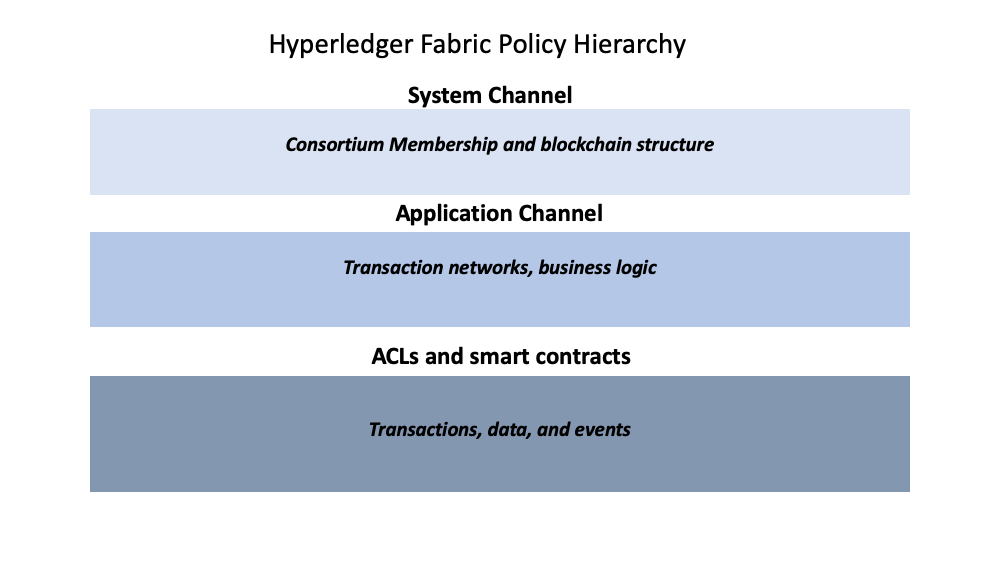
\includegraphics[width=1\textwidth]{img/policy-hierarchy.png}
    \caption{Livelli della gerarchia delle policy in Hyperledger Fabric}
    \label{fig:policy-fabric}
\end{figure}
\paragraph{Configurazione del canale di sistema}
Una delle prime configurazioni prima del caricamento della rete è quella legata al canale di sistema. Tale canale è unico, contiene le organizzazioni legate al servizio di ordinamento e le organizzazioni del consorzio, ossia quelle capaci di effettuare delle transazioni all'interno della rete. Le politiche di configurazione che interessano il canale di sistema regolano il meccanismo del consenso proprio del sistema di ordinamento e la modalità di creazione e di formattazione di un nuovo blocco e, infine, regola anche i membri del consorzio capaci di creare un canale all'interno della rete blockchain.
\paragraph{Configurazione del canale applicativo}
La configurazione di un canale applicativo definisce una comunicazione privata tra alcune organizzazioni del consorzio. Le policy legate a tale configurazioni definiscono la gestione dell'aggiunta o della rimozione di un membro all'interno del canale, definisce anche quali organizzazioni siano necessarie per la validazione dei chaincode prima che questi siano sottomessi definitivamente al commit. Quando un canale viene creato, esso eredita per default tutte le caratteristiche del canale di sistema. I parametri che definiscono la gestione delle operazioni di manipolazione di risorse del canale possono essere personalizzate secondo le regole di configurazione dei canali applicativi.
\paragraph{Configurazione degli ACL e dei smart contract}
La configurazione degli ACL definisce la lista di controllo degli accessi ad una determinata risorsa, ossia quali membri possono accederci. Tramite gli ACL è possibile definire, cosi, la visibilità di una particolare risorsa. Gli amministratori di sistema definiscono la configurazione di tali liste attraverso delle politiche dedicate. Dentro tali regole, è possibile definire l'accessibilità a funzioni di chaincode, a strutture dati oppure ai valori degli oggetti dello stato globale del ledger distribuito. La configurazione di un ACL definisce i criteri di aggiornamento delle risorse proprie di un canale applicativo. Le risorse all'interno delle ACL visibili all'interno della rete su particolari canali applicativi sono mantenuti dentro un file policy specifico chiamato configtx.yaml.
Per quanto riguarda le politiche di gestione del chaincode, esse vengono definite durante la creazione del chaincode stesso e durano per tutto il ciclo di vita del chaincode. Essa può essere definita per default all'interno della configurazione del canale su cui viene caricato, oppure dentro un file specifico che definisce la politica di approvazione del chaincode in cui sono mantenuti i criteri quali la gestione dell'ordinamento e della validazione di una transazione.
\newpage
\section{Dati privati}
Con dati privati andiamo a identificare tutte quelle informazioni che possono essere visibili solamente a un sottoinsieme di account della rete. Nel caso specifico delle blockchain basate su Fabric, tale obiettivo può essere raggiunto andando a definire dei canali dedicati per la visibilità di alcuni tipi di strutture dati. Questa soluzione, però, può causare dei problemi per il sovraccarico dei processi amministrativi della rete (gestione di chaincode multipli, criteri da rispettare, MSP...). Per questo motivo, Hyperledger Fabric dispone di meccanismi in grado di stabilire dei dati privati che sono visibili e gestibili da un sottoinsieme specifico di organizzazioni.
Una collezione di dati è in genere costituita da due elementi:
\newpage
\begin{enumerate}
\item I dati correnti: Mantenuti all'interno di un database di stato corrente distribuito ai vari peer delle organizzazioni autorizzate alla visualizzazione e alla manipolazione di tali strutture mediante l'utilizzo delle istanze dei chaincode proprie di un peer.
\item Un hash dati: In modo da tenere traccia e convalidare le transazioni proprie per quell'insieme di valori e utilizzarle anche per altri scopi legati alla logica di business che si vuole implementare. Notiamo che tale hash ha solamente un riferimento ai dati senza avere nessun collegamento reale.
\end{enumerate}
In seguito riportiamo una figura che rappresenta la differente visione dei dati per un peer di un'organizzazione autorizzata rispetto a un peer di un'altra organizzazione senza diritti di gestione.
\begin{figure}[h]
    \centering
    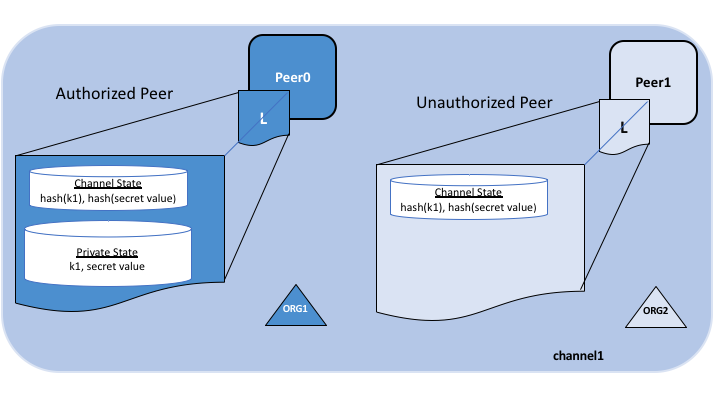
\includegraphics[width=1\textwidth]{img/data-private-vision.png}
    \caption{Gestione della visione dei dati privati}
    \label{fig:private-data}
\end{figure}
I membri della raccolta possono decidere di condividere i dati privati con terze parti, se vogliono trasferire l'asset delle informazioni a nodi esterni al dominio di visibilità dei dati. Le terze parti interessate possono calcolare l'hash dei dati privati e vedere se corrispondano allo stato del libro mastro del canale, cosi dapoter verificarne l'esistenza nel contesto visibile ai membri della collezione.
In molti casi vediamo che le organizzazioni possiedono delle proprie collezioni private che possano essere condivise successivamente a peer di altre organizzazioni tramite la creazione di transazioni che invochino funzionalità del chaincode installato sul canale.
\subsection{Composizione della transazione per i dati privati}
Quando si fa riferimento a raccolte di dati privati dei chaincode, il flusso delle transazioni è leggermente diverso per le proposte, approvazione e l'inserimento nel ledger.
Il flusso di esecuzione che si esegue per tale tipo di transazioni è il seguente:
\begin{enumerate}
    \item L'applicazione client inoltra una richiesta di proposta di transazione per invocare una funzione chaincode (lettura o scrittura di dati privati) per garantire l'approvazione dei peer che fanno parte delle organizzazioni autorizzate della collezione degli asset privati. I dati privati, o i dati utilizzati per generare dati privati in chaincode, vengono inviati in un campo transitorio della proposta di transazione. 
    \item I peer legati alle politiche di approvazione della proposta di transazione eseguono una simulazione della transazione andando a memorizzare lo stato risultante all'interno di registri temporanei e propagano i dati agli altri peer secondo le politiche legate alla configurazione della collezione dei dati privati presa sotto esame. 
    \item I peer di approvazione inviano una risposta al client strutturata come un set di lettura / scrittura andando a mandare l'hash per i riferimenti ai dati privati e i valori risultati reali per i dati pubblici cosi da mantenere un criterio di riservatezza finchè non si è validata la transazione. 
    \item La proposta di transazione verrà rimandata insieme alla transazione effettiva al servizio di ordinamento che includerà gli hash dei dati privati all'interno del blocco di transazione. Tale blocco verrà distribuito a tutti i peer. In questo modo, ogni peer può convalidare il blocco di transazione utilizzando i soli hash di dati privati senza accedere ai loro valori effettivi.
    \item Al momento del commit del blocco, i peer autorizzati utilizzano le politiche di configurazione della collezione per determinare se sono autorizzati ad avere accesso ai dati privati. In caso affermativo, per prima cosa controlleranno il loro archivio di dati transitori locali per determinare se hanno già ricevuto i dati privati durante la proposta di transazione sulle funzionalità richiamate dal chaincode. In caso contrario, tenteranno di estrarre i dati privati da un altro peer autorizzato per poi convalidarli. Al momento della convalida, i dati privati vengono spostati nella loro copia del database in cui è memorizzato lo stato privato della collezione. Infine, una volta terminata la transazione, i dati privati contenuti all'interno dei registri temporanei vengono eliminati. 
\end{enumerate}
\subsection{Politiche di configurazione per i dati privati}
Una delle principali caratteristiche che rappresentano la gestione dei dati privati all'interno di Fabric è rappresentata dai criteri di configurazione delle collezioni privati. In questo contesto, vi si scandiscono alcune proprietà fondamentali capaci di determinare la gestione delle collezioni all'interno dei vari peer della rete in relazione alle richieste di applicazioni client esterne.
La definizione delle collezioni (pubbliche e private), sono mantenute all'interno di un file di configurazione formattato in un array di JSON. Ogni elemento dell'array rappresenta una configurazione della gestione di una struttura dati definita internamente a un chaincode di un canale della rete.
Le proprietà principali delle collezioni sono le seguenti:
\begin{enumerate}
     \item name: Nome della collezione
    \item policy: Rappresentano dei criteri di configurazione della distribuzione delle collezioni private in cui definiscono quali organizzazioni possono accedere ai valori della struttura dati rappresentata dalla collezione. Si utilizza una sintassi basata su una firma OR in cui si definisce tra parentesi le organizzazioni e quali componenti di tali organizzazioni possono effettuare delle operazioni sulla collezione specificata.
    \item requiredPeerCount: Numero di peer delle organizzazioni autorizzate che devono ricevere i dati privati per il processo di convalida della proposta di transazione prima di restituirne una risposta all'applicazione client.
    \item maxPeerCount: Numero di peer massimo tra quelli delle organizzazioni autorizzate per la validazione della proposta di transazione, tale caratteristica è alla base del criterio di ridondanza che mantiene un grado di affidabilità sempre accettabile anche se alcuni peer che sono interessati nel processo di consenso non sono momentaneamente disponibili.
    \item blockToLive: Definisce il numero di blocchi successivi che devono essere creati prima dell'eliminazione dei valori di uno stato mantenuto all'interno di un blocco. Questa proprietà è importante poichè serve ad eliminare blocchi di dati obsoleti. Se si vuole mantenere persistente un blocco in cui è mantenuta una istanza della collezione, tale valore viene impostato a 0.
    \item memberOnlyRead: Se impostata a true, solamente i membri delle organizzazioni dichiarati nelle politiche di distribuzione della collezioni hanno la possibilità di leggere delle informazioni dalla collezione. Nel caso in cui si intenda invocare il chaincode su una funzione di lettura e non si è parte delle organizzazioni a cui si sottopongono questi criteri, l'invocazione ritornerà uno status di errore.
    \item memberOnlyWrite: Se impostato a true, come per la proprietà di memberOnlyRead, definisce una limitazione di scrittura solamente ai membri delle organizzazioni dichiarate nelle politiche di distribuzione della collezione. Quindi l'invocazione di funzioni del chaincode che prevedono un'operazione di scrittura, torneranno un errore se i membri che invocano tale operazioni fanno parte di una organizzazione non autorizzata.
    \item endorsementPolicy: Stabilisce dei criteri che vanno a sovrascrivere quelli del canale in cui è installato il chaincode di riferimento. In questo caso è possibile stabilire un insieme di organizzazione per il consenso e la convalida delle proposte di transazioni differenti rispetto a quelle stabilisce dal canale.
\end{enumerate}
\newpage